\subsection{Pusher-v5 PPO-TV}
Thirty training seeds per setting. Bands are one sample SD across policy means, not confidence intervals. Ordinary standard is fixed; the best complete parameter is selected ex post separately per axis. All eight declared caps complete; 20 episodes per condition; matched competent-training recipe, not a physical-success certificate.
\begin{figure}[p]\centering
\begin{subfigure}{0.48\textwidth}\centering
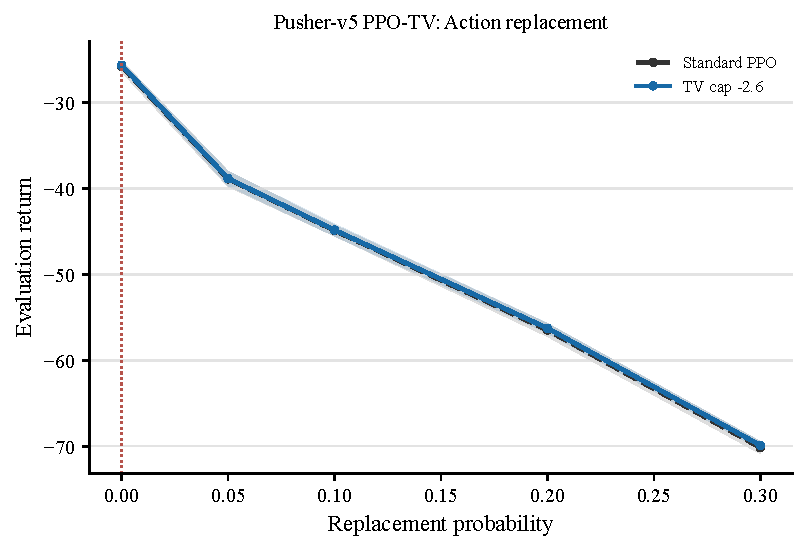
\includegraphics[width=\linewidth]{plots/pusher_ppo_tv30/action_replacement.pdf}
\caption{Action replacement}
\end{subfigure}\hfill
\begin{subfigure}{0.48\textwidth}\centering
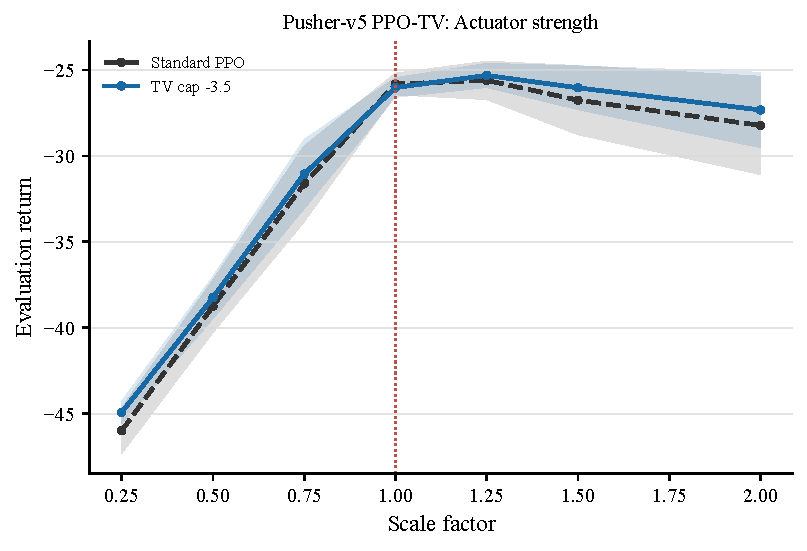
\includegraphics[width=\linewidth]{plots/pusher_ppo_tv30/actuator_strength.pdf}
\caption{Actuator strength}
\end{subfigure}\par\medskip
\begin{subfigure}{0.48\textwidth}\centering
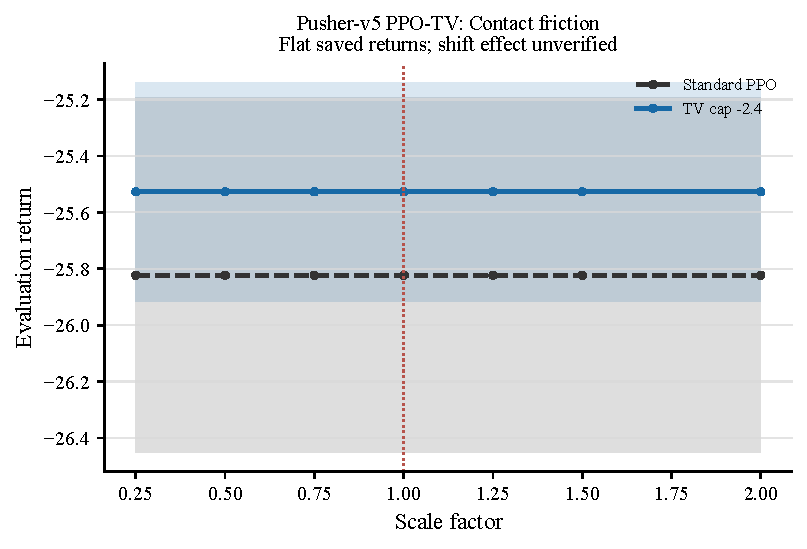
\includegraphics[width=\linewidth]{plots/pusher_ppo_tv30/friction.pdf}
\caption{Contact friction}
\end{subfigure}\hfill
\begin{subfigure}{0.48\textwidth}\centering
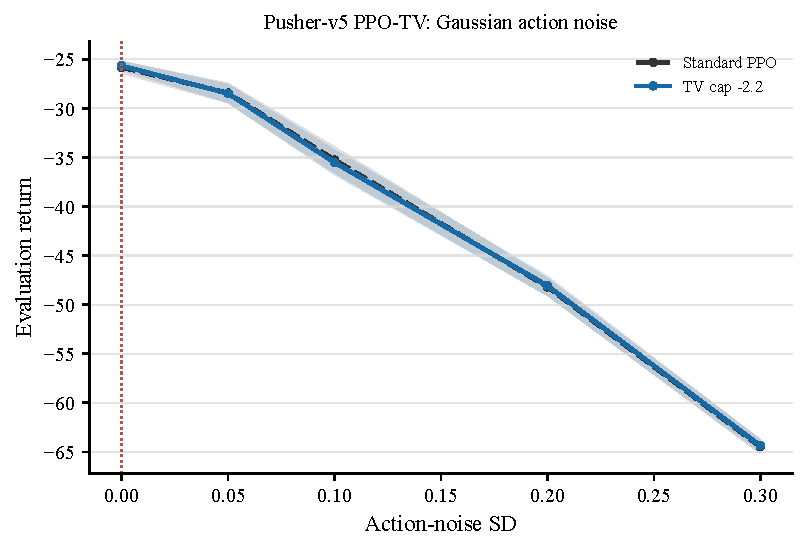
\includegraphics[width=\linewidth]{plots/pusher_ppo_tv30/gaussian_action_noise.pdf}
\caption{Gaussian action noise}
\end{subfigure}\par\medskip
\caption{Pusher-v5 PPO-TV. Mean and sample SD across 30 training seeds; ex-post selection.}
\end{figure}
\begin{figure}[p]\centering
\begin{subfigure}{0.48\textwidth}\centering
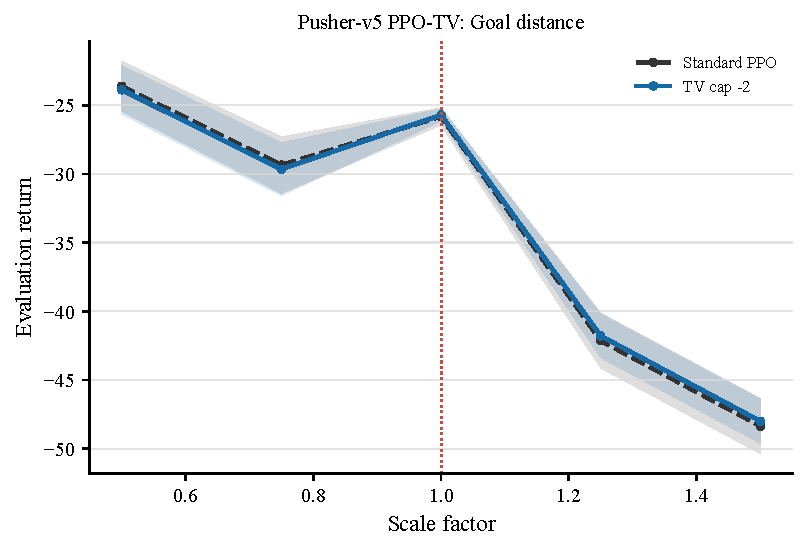
\includegraphics[width=\linewidth]{plots/pusher_ppo_tv30/goal_distance.pdf}
\caption{Goal distance}
\end{subfigure}\hfill
\begin{subfigure}{0.48\textwidth}\centering
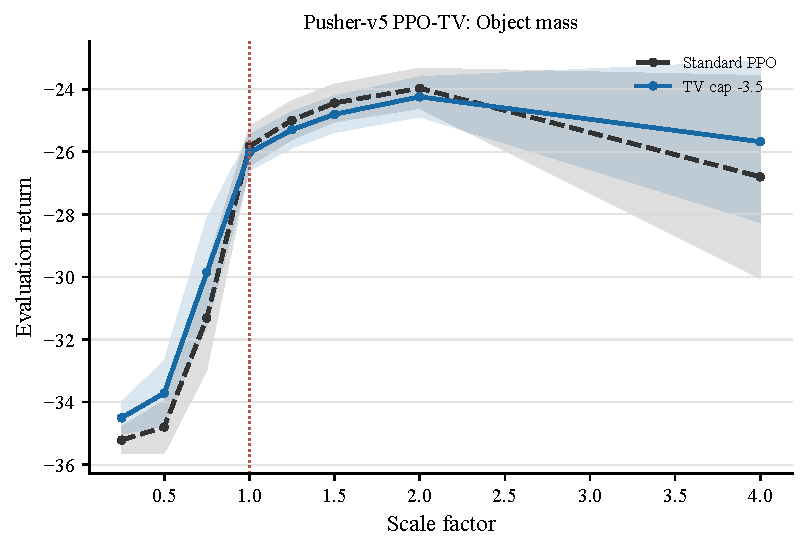
\includegraphics[width=\linewidth]{plots/pusher_ppo_tv30/object_mass.pdf}
\caption{Object mass}
\end{subfigure}\par\medskip
\caption{Pusher-v5 PPO-TV. Mean and sample SD across 30 training seeds; ex-post selection.}
\end{figure}
\subsection{Pusher-v5 SAC-TV}
Thirty training seeds per setting. Bands are one sample SD across policy means, not confidence intervals. Ordinary standard is fixed; the best complete parameter is selected ex post separately per axis. All eight declared caps complete; 20 episodes per condition; matched competent-training recipe, not a physical-success certificate.
\begin{figure}[p]\centering
\begin{subfigure}{0.48\textwidth}\centering
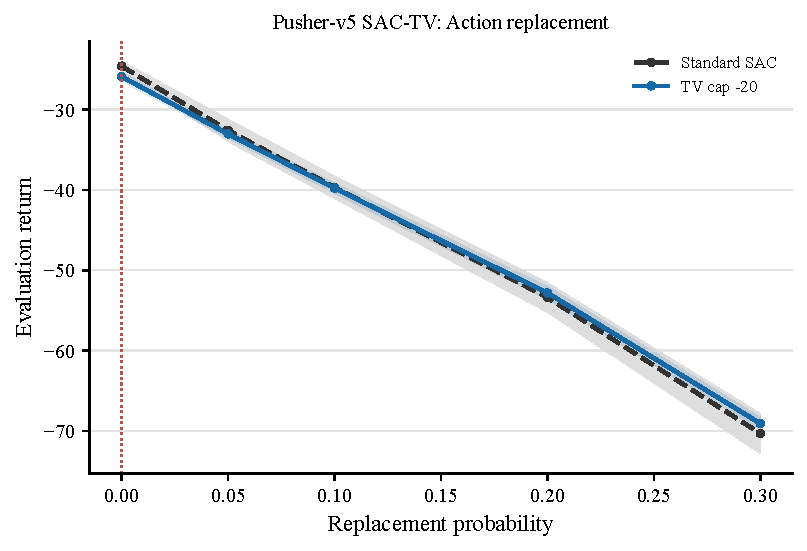
\includegraphics[width=\linewidth]{plots/pusher_sac_tv30/action_replacement.pdf}
\caption{Action replacement}
\end{subfigure}\hfill
\begin{subfigure}{0.48\textwidth}\centering
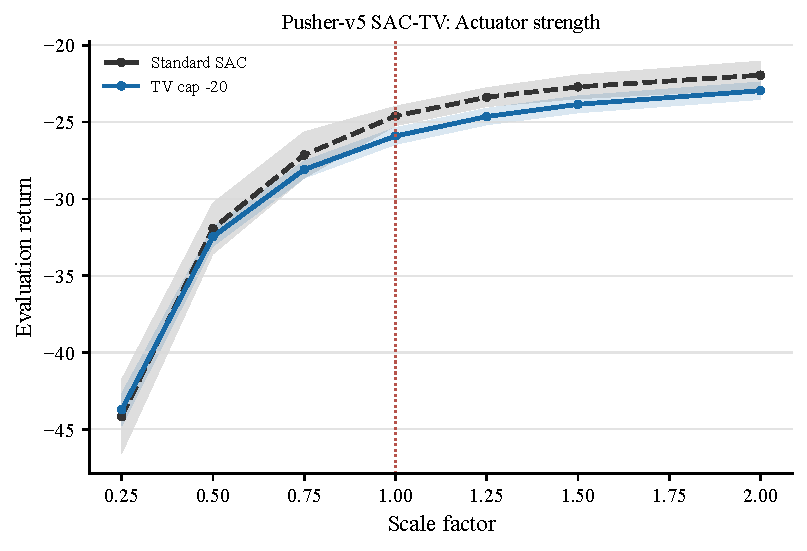
\includegraphics[width=\linewidth]{plots/pusher_sac_tv30/actuator_strength.pdf}
\caption{Actuator strength}
\end{subfigure}\par\medskip
\begin{subfigure}{0.48\textwidth}\centering
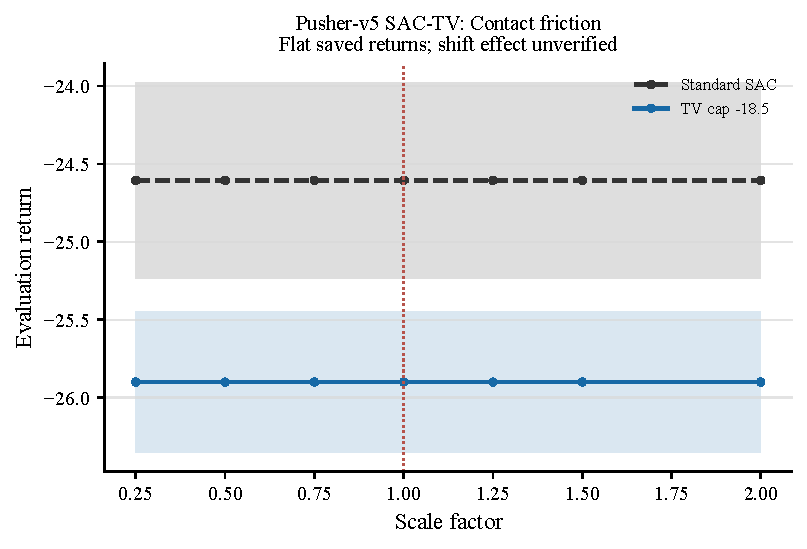
\includegraphics[width=\linewidth]{plots/pusher_sac_tv30/friction.pdf}
\caption{Contact friction}
\end{subfigure}\hfill
\begin{subfigure}{0.48\textwidth}\centering
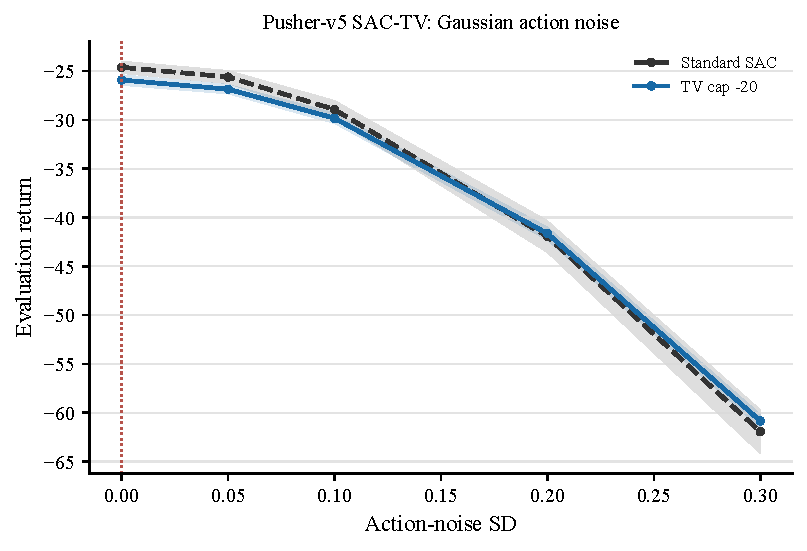
\includegraphics[width=\linewidth]{plots/pusher_sac_tv30/gaussian_action_noise.pdf}
\caption{Gaussian action noise}
\end{subfigure}\par\medskip
\caption{Pusher-v5 SAC-TV. Mean and sample SD across 30 training seeds; ex-post selection.}
\end{figure}
\begin{figure}[p]\centering
\begin{subfigure}{0.48\textwidth}\centering
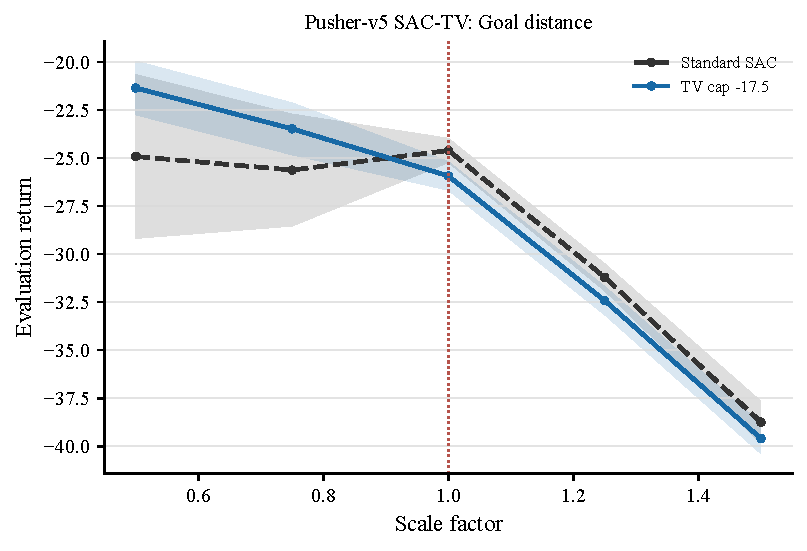
\includegraphics[width=\linewidth]{plots/pusher_sac_tv30/goal_distance.pdf}
\caption{Goal distance}
\end{subfigure}\hfill
\begin{subfigure}{0.48\textwidth}\centering
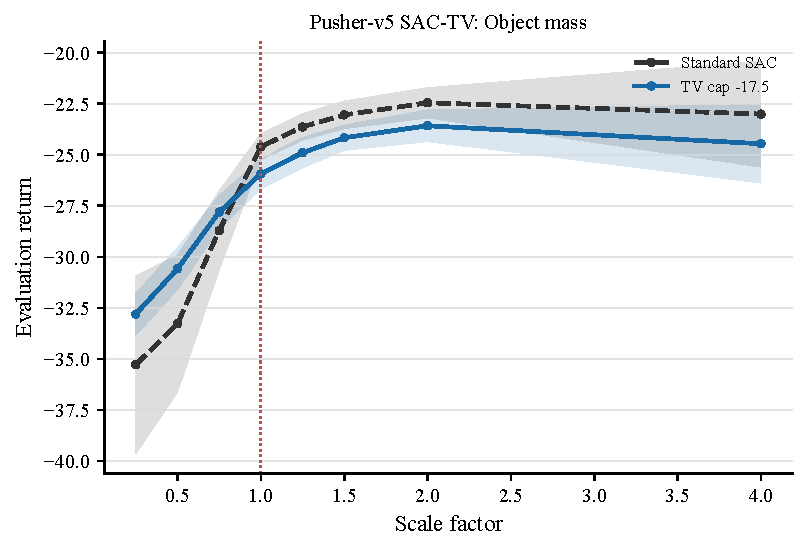
\includegraphics[width=\linewidth]{plots/pusher_sac_tv30/object_mass.pdf}
\caption{Object mass}
\end{subfigure}\par\medskip
\caption{Pusher-v5 SAC-TV. Mean and sample SD across 30 training seeds; ex-post selection.}
\end{figure}
\subsection{Pusher-v5 TD3-TV}
Thirty training seeds per setting. Bands are one sample SD across policy means, not confidence intervals. Ordinary standard is fixed; the best complete parameter is selected ex post separately per axis. All eight declared caps complete; 20 episodes per condition; matched competent-training recipe, not a physical-success certificate.
\begin{figure}[p]\centering
\begin{subfigure}{0.48\textwidth}\centering
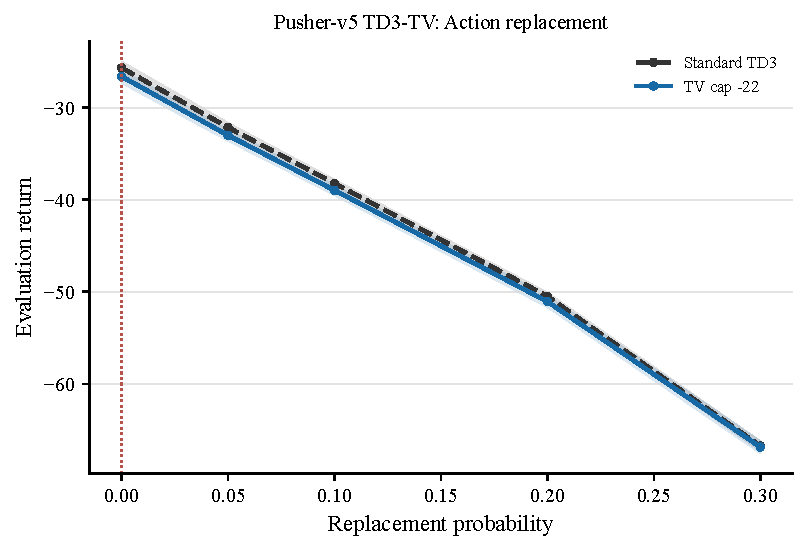
\includegraphics[width=\linewidth]{plots/pusher_td3_tv30/action_replacement.pdf}
\caption{Action replacement}
\end{subfigure}\hfill
\begin{subfigure}{0.48\textwidth}\centering
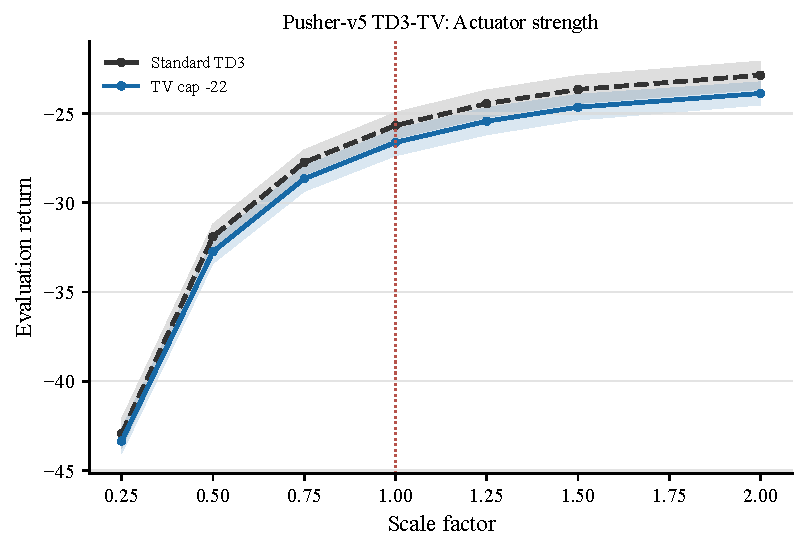
\includegraphics[width=\linewidth]{plots/pusher_td3_tv30/actuator_strength.pdf}
\caption{Actuator strength}
\end{subfigure}\par\medskip
\begin{subfigure}{0.48\textwidth}\centering
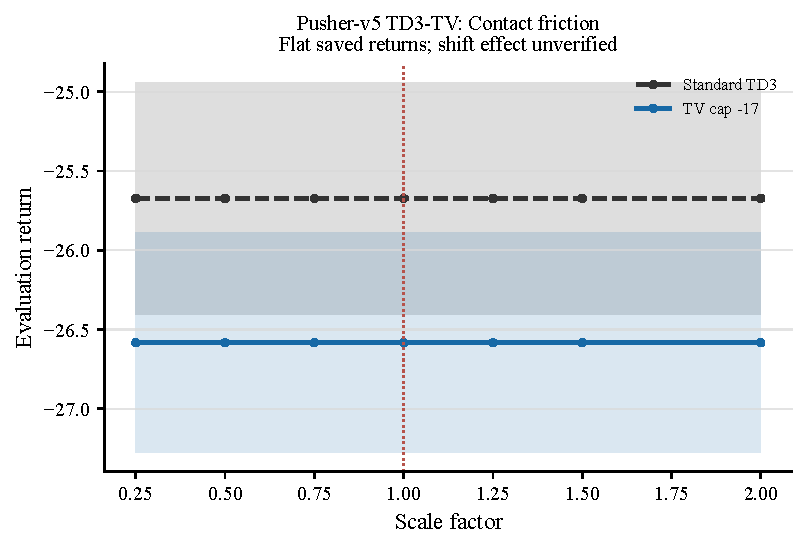
\includegraphics[width=\linewidth]{plots/pusher_td3_tv30/friction.pdf}
\caption{Contact friction}
\end{subfigure}\hfill
\begin{subfigure}{0.48\textwidth}\centering
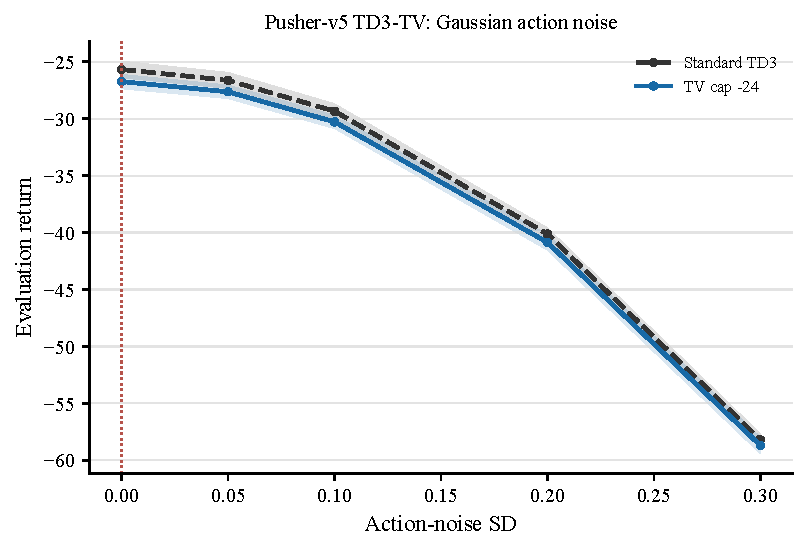
\includegraphics[width=\linewidth]{plots/pusher_td3_tv30/gaussian_action_noise.pdf}
\caption{Gaussian action noise}
\end{subfigure}\par\medskip
\caption{Pusher-v5 TD3-TV. Mean and sample SD across 30 training seeds; ex-post selection.}
\end{figure}
\begin{figure}[p]\centering
\begin{subfigure}{0.48\textwidth}\centering
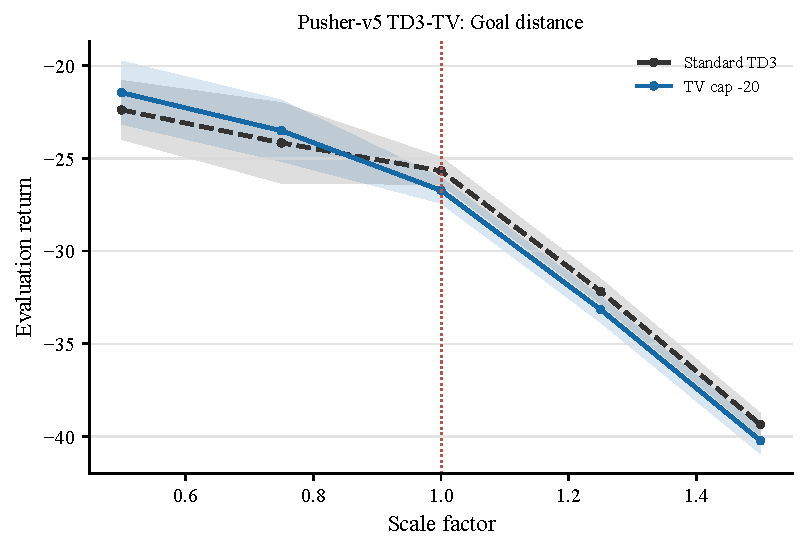
\includegraphics[width=\linewidth]{plots/pusher_td3_tv30/goal_distance.pdf}
\caption{Goal distance}
\end{subfigure}\hfill
\begin{subfigure}{0.48\textwidth}\centering
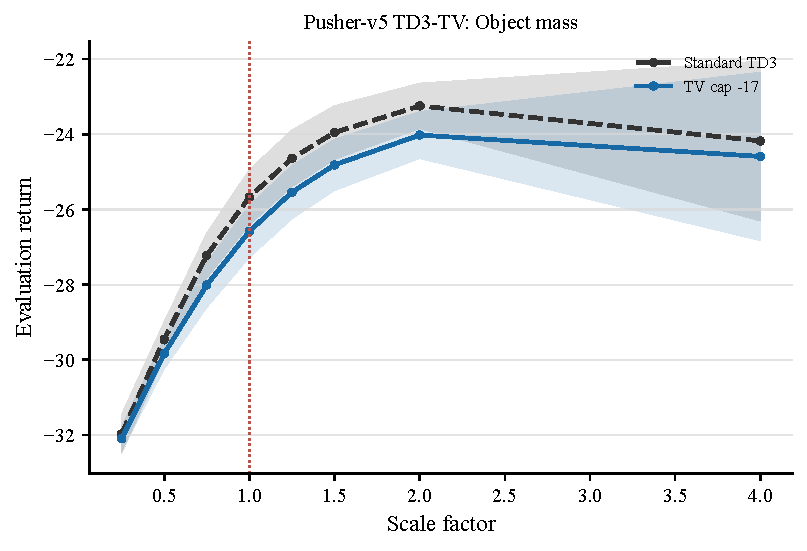
\includegraphics[width=\linewidth]{plots/pusher_td3_tv30/object_mass.pdf}
\caption{Object mass}
\end{subfigure}\par\medskip
\caption{Pusher-v5 TD3-TV. Mean and sample SD across 30 training seeds; ex-post selection.}
\end{figure}
\subsection{ANYmal PPO-TV}
Thirty training seeds per setting. Bands are one sample SD across policy means, not confidence intervals. Ordinary standard is fixed; the best complete parameter is selected ex post separately per axis. 4/7 declared TV caps have full 30-seed suites; 29,491,200 native transitions per policy. Competence not certified by returns/completion.
\begin{figure}[p]\centering
\begin{subfigure}{0.48\textwidth}\centering
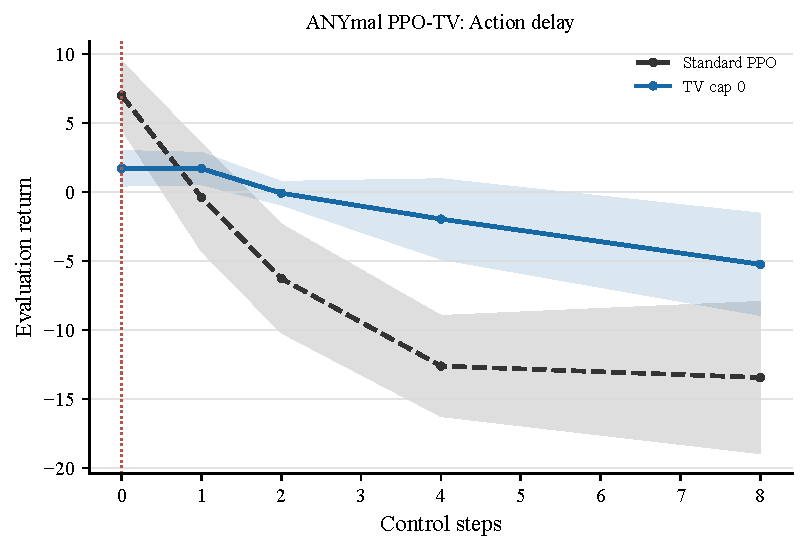
\includegraphics[width=\linewidth]{plots/anymal_ppo_tv30/action_delay.pdf}
\caption{Action delay}
\end{subfigure}\hfill
\begin{subfigure}{0.48\textwidth}\centering
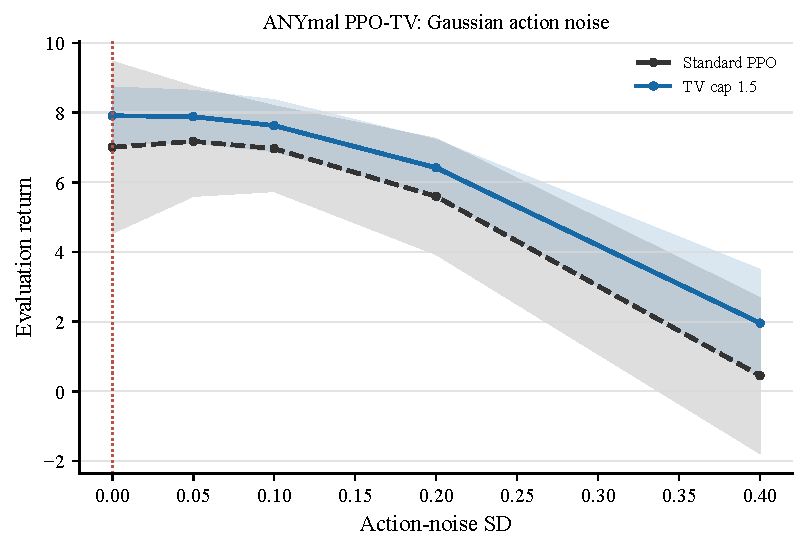
\includegraphics[width=\linewidth]{plots/anymal_ppo_tv30/action_noise.pdf}
\caption{Gaussian action noise}
\end{subfigure}\par\medskip
\begin{subfigure}{0.48\textwidth}\centering
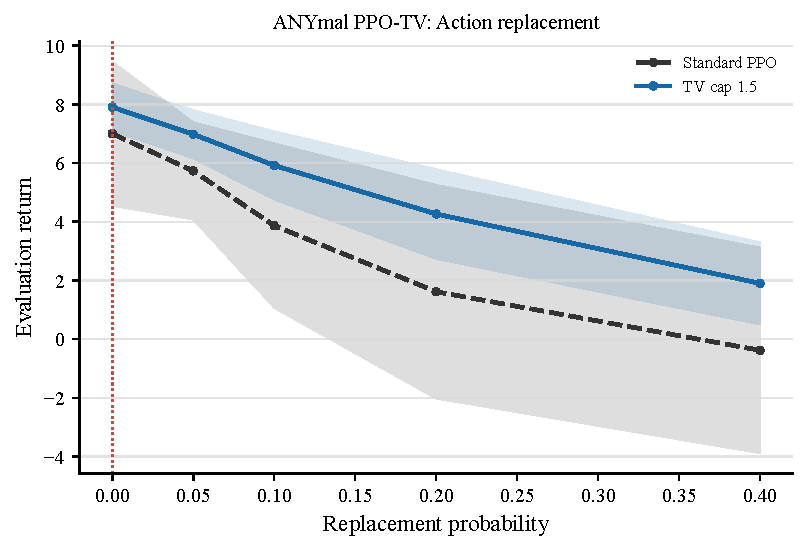
\includegraphics[width=\linewidth]{plots/anymal_ppo_tv30/action_replacement.pdf}
\caption{Action replacement}
\end{subfigure}\hfill
\begin{subfigure}{0.48\textwidth}\centering
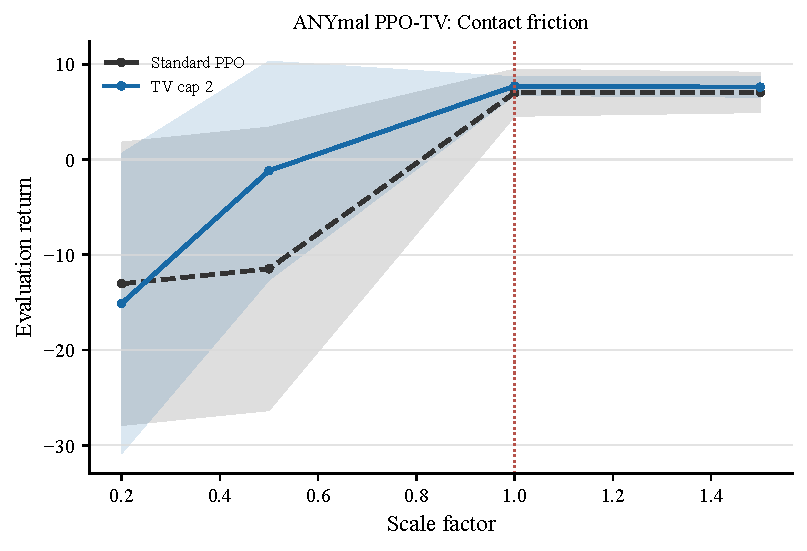
\includegraphics[width=\linewidth]{plots/anymal_ppo_tv30/contact_friction.pdf}
\caption{Contact friction}
\end{subfigure}\par\medskip
\caption{ANYmal PPO-TV. Mean and sample SD across 30 training seeds; ex-post selection.}
\end{figure}
\begin{figure}[p]\centering
\begin{subfigure}{0.48\textwidth}\centering
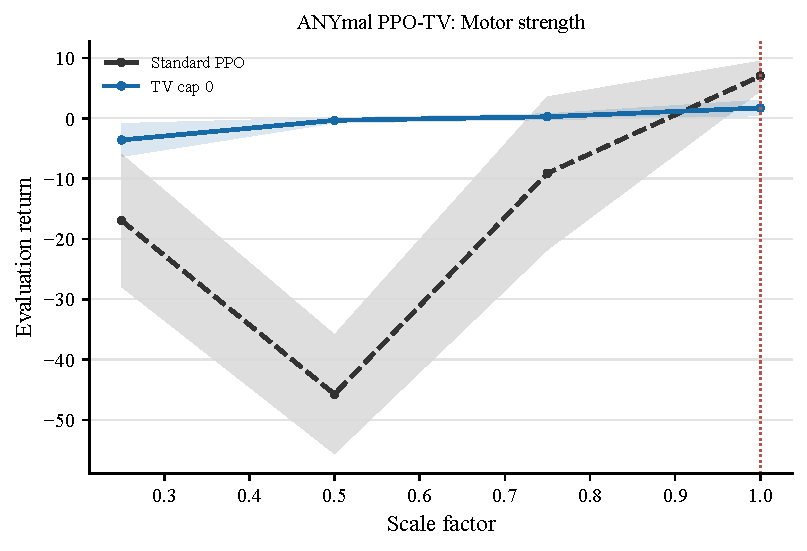
\includegraphics[width=\linewidth]{plots/anymal_ppo_tv30/motor_strength.pdf}
\caption{Motor strength}
\end{subfigure}\hfill
\begin{subfigure}{0.48\textwidth}\centering
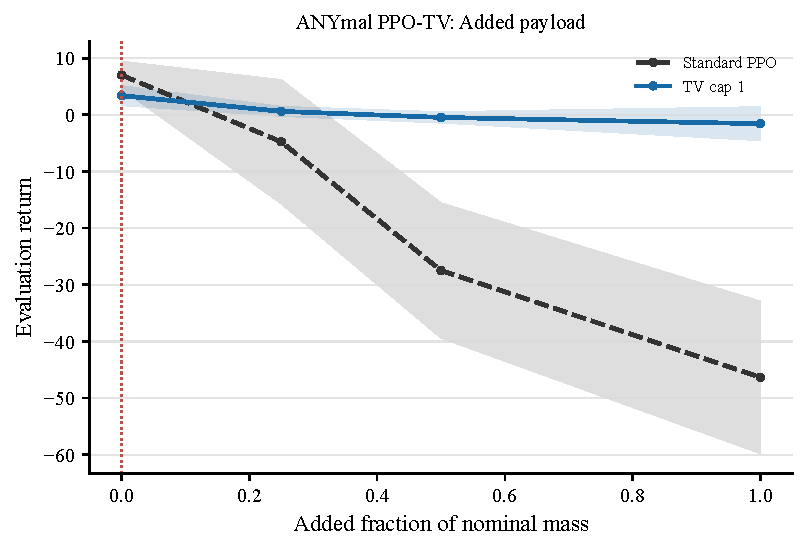
\includegraphics[width=\linewidth]{plots/anymal_ppo_tv30/payload_fraction.pdf}
\caption{Added payload}
\end{subfigure}\par\medskip
\caption{ANYmal PPO-TV. Mean and sample SD across 30 training seeds; ex-post selection.}
\end{figure}
\subsection{Ant SAC-TV}
Thirty training seeds per setting. Bands are one sample SD across policy means, not confidence intervals. Ordinary standard is fixed; the best complete parameter is selected ex post separately per axis. 6/6 declared TV caps have full 30-seed suites; 512,000 native transitions per policy. Competence not certified by returns/completion.
\begin{figure}[p]\centering
\begin{subfigure}{0.48\textwidth}\centering
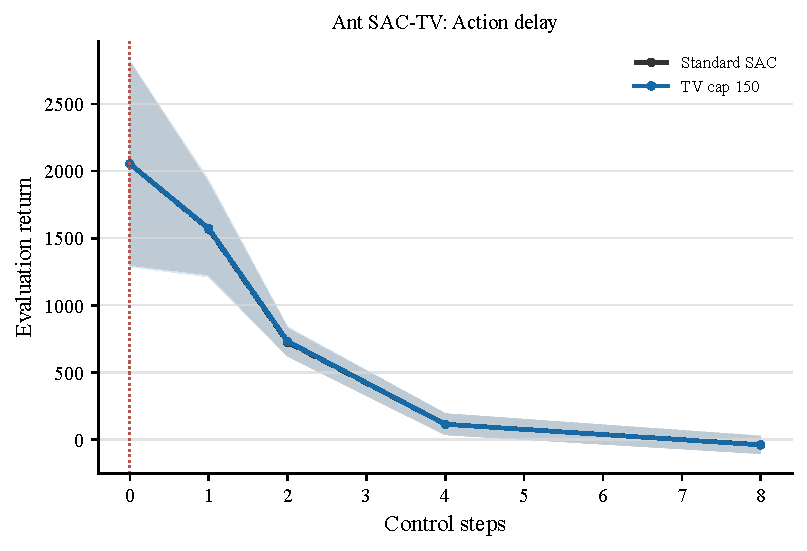
\includegraphics[width=\linewidth]{plots/ant_sac_tv30/action_delay.pdf}
\caption{Action delay}
\end{subfigure}\hfill
\begin{subfigure}{0.48\textwidth}\centering
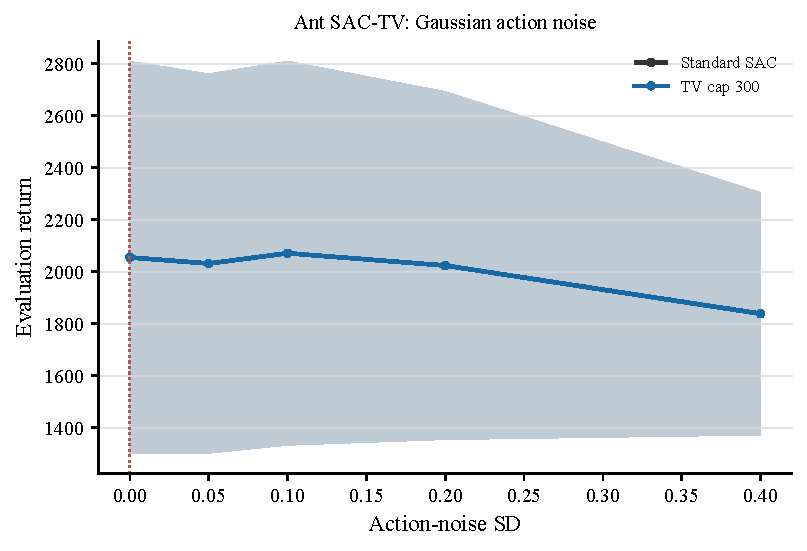
\includegraphics[width=\linewidth]{plots/ant_sac_tv30/action_noise.pdf}
\caption{Gaussian action noise}
\end{subfigure}\par\medskip
\begin{subfigure}{0.48\textwidth}\centering
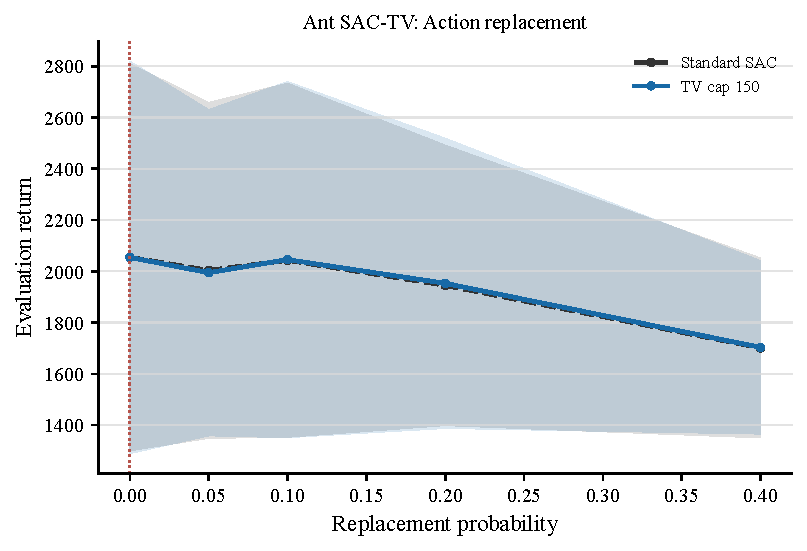
\includegraphics[width=\linewidth]{plots/ant_sac_tv30/action_replacement.pdf}
\caption{Action replacement}
\end{subfigure}\hfill
\begin{subfigure}{0.48\textwidth}\centering
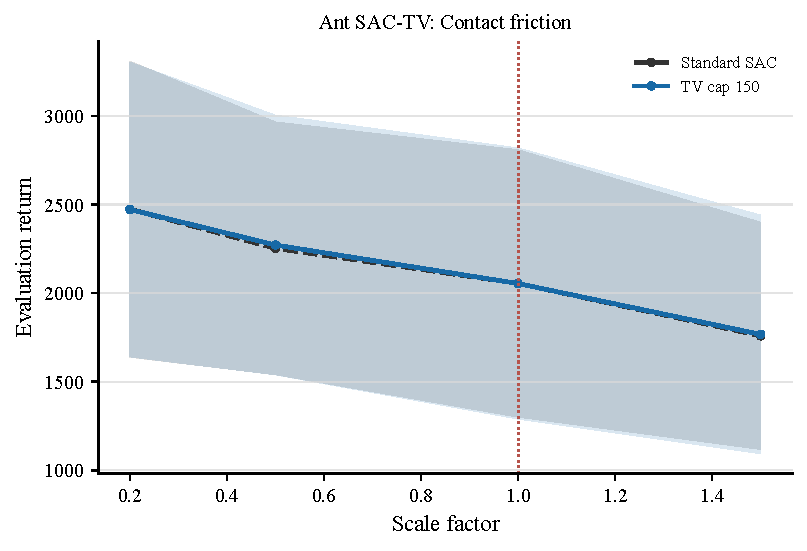
\includegraphics[width=\linewidth]{plots/ant_sac_tv30/contact_friction.pdf}
\caption{Contact friction}
\end{subfigure}\par\medskip
\caption{Ant SAC-TV. Mean and sample SD across 30 training seeds; ex-post selection.}
\end{figure}
\begin{figure}[p]\centering
\begin{subfigure}{0.48\textwidth}\centering
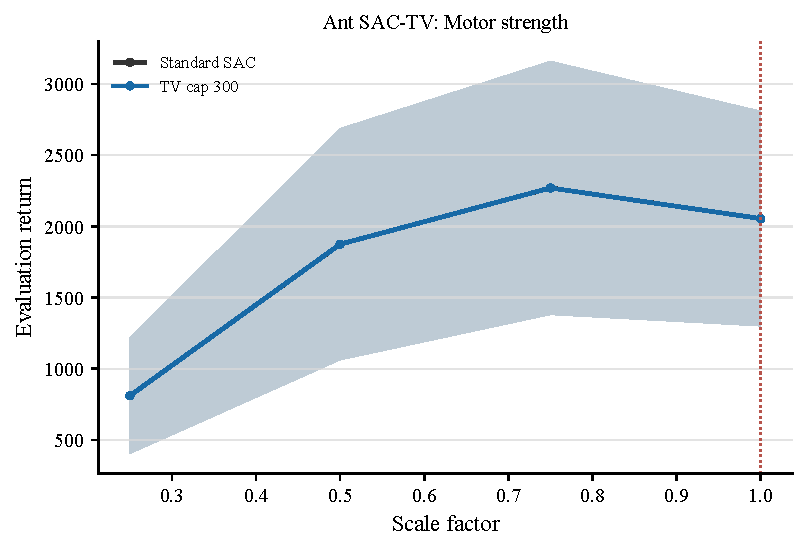
\includegraphics[width=\linewidth]{plots/ant_sac_tv30/motor_strength.pdf}
\caption{Motor strength}
\end{subfigure}\hfill
\begin{subfigure}{0.48\textwidth}\centering
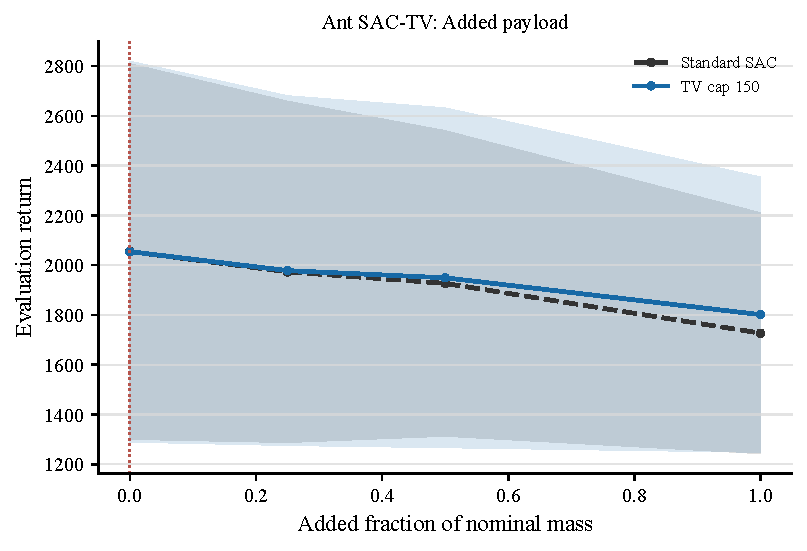
\includegraphics[width=\linewidth]{plots/ant_sac_tv30/payload_fraction.pdf}
\caption{Added payload}
\end{subfigure}\par\medskip
\caption{Ant SAC-TV. Mean and sample SD across 30 training seeds; ex-post selection.}
\end{figure}
\subsection{Ant TD3-TV}
Thirty training seeds per setting. Bands are one sample SD across policy means, not confidence intervals. Ordinary standard is fixed; the best complete parameter is selected ex post separately per axis. 2/6 declared TV caps have full 30-seed suites; 512,000 native transitions per policy. Competence not certified by returns/completion.
\begin{figure}[p]\centering
\begin{subfigure}{0.48\textwidth}\centering
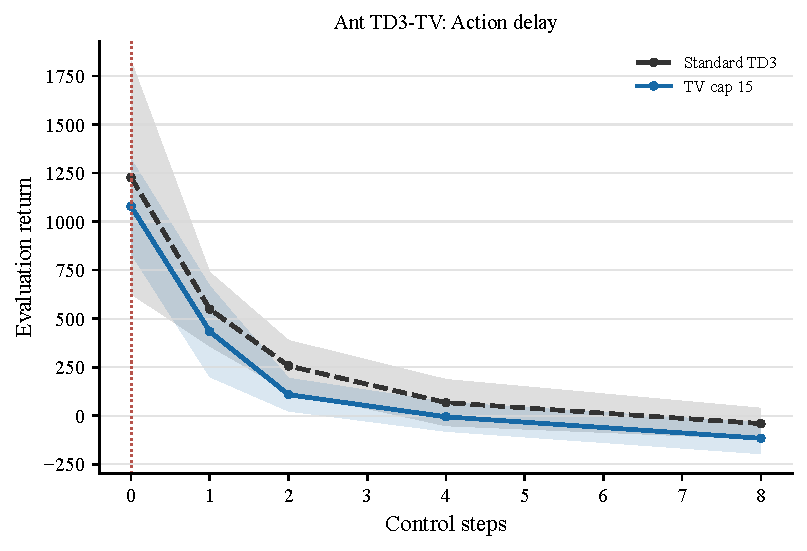
\includegraphics[width=\linewidth]{plots/ant_td3_tv30/action_delay.pdf}
\caption{Action delay}
\end{subfigure}\hfill
\begin{subfigure}{0.48\textwidth}\centering
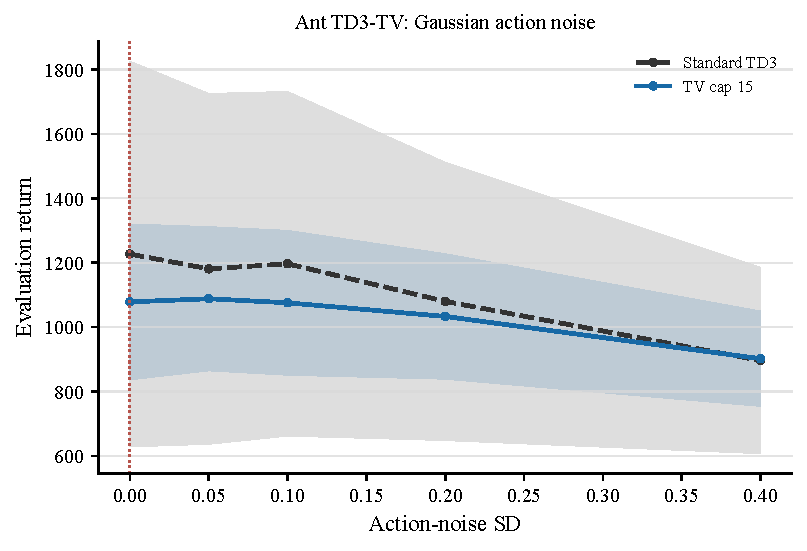
\includegraphics[width=\linewidth]{plots/ant_td3_tv30/action_noise.pdf}
\caption{Gaussian action noise}
\end{subfigure}\par\medskip
\begin{subfigure}{0.48\textwidth}\centering
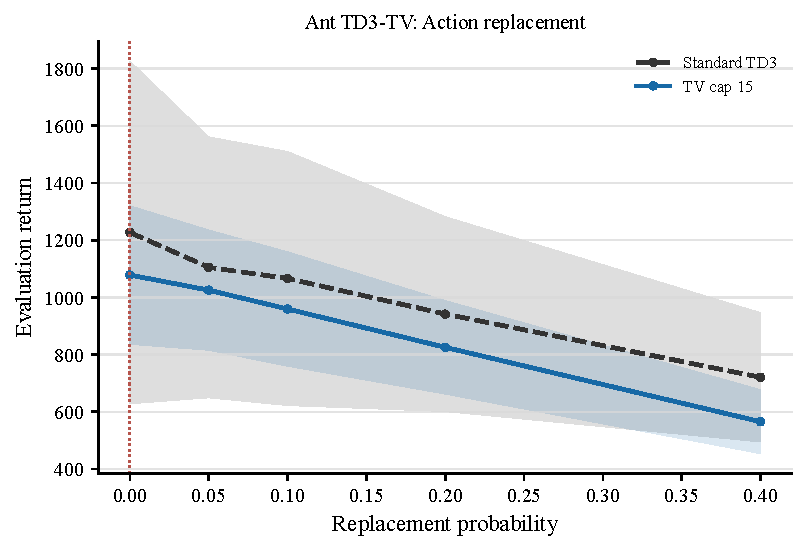
\includegraphics[width=\linewidth]{plots/ant_td3_tv30/action_replacement.pdf}
\caption{Action replacement}
\end{subfigure}\hfill
\begin{subfigure}{0.48\textwidth}\centering
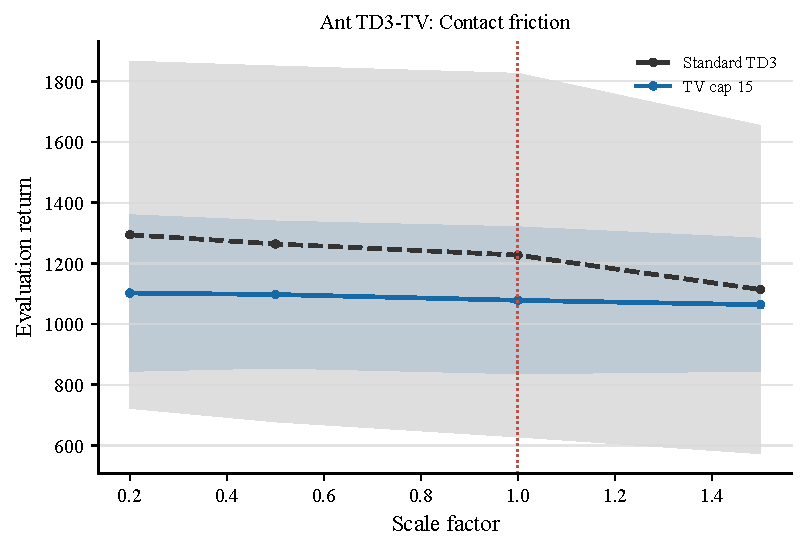
\includegraphics[width=\linewidth]{plots/ant_td3_tv30/contact_friction.pdf}
\caption{Contact friction}
\end{subfigure}\par\medskip
\caption{Ant TD3-TV. Mean and sample SD across 30 training seeds; ex-post selection.}
\end{figure}
\begin{figure}[p]\centering
\begin{subfigure}{0.48\textwidth}\centering
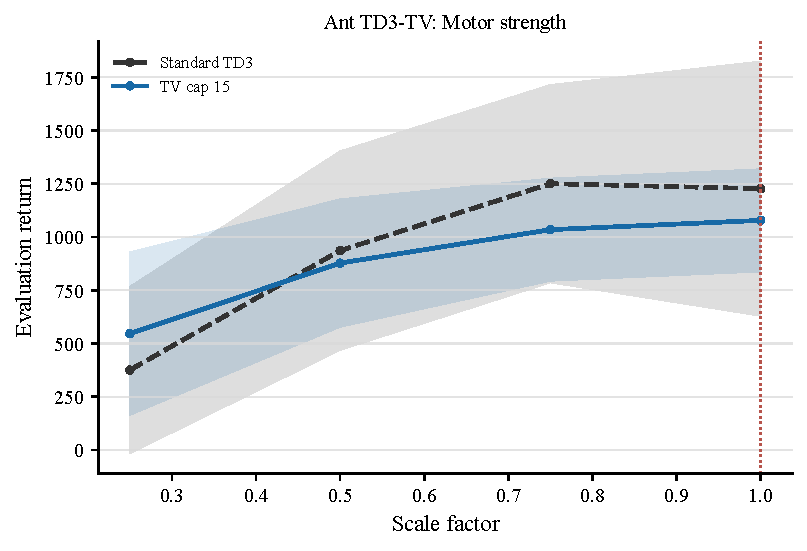
\includegraphics[width=\linewidth]{plots/ant_td3_tv30/motor_strength.pdf}
\caption{Motor strength}
\end{subfigure}\hfill
\begin{subfigure}{0.48\textwidth}\centering
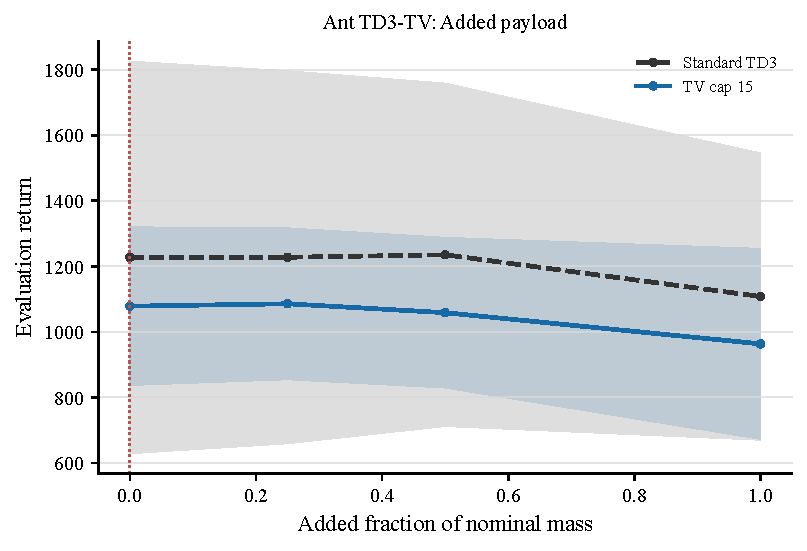
\includegraphics[width=\linewidth]{plots/ant_td3_tv30/payload_fraction.pdf}
\caption{Added payload}
\end{subfigure}\par\medskip
\caption{Ant TD3-TV. Mean and sample SD across 30 training seeds; ex-post selection.}
\end{figure}
\subsection{Drawer PPO-TV}
Thirty training seeds per setting. Bands are one sample SD across policy means, not confidence intervals. Ordinary standard is fixed; the best complete parameter is selected ex post separately per axis. 1/6 declared TV caps have full 30-seed suites; 10,240,000 native transitions per policy. Competence not certified by returns/completion.
\begin{figure}[p]\centering
\begin{subfigure}{0.48\textwidth}\centering
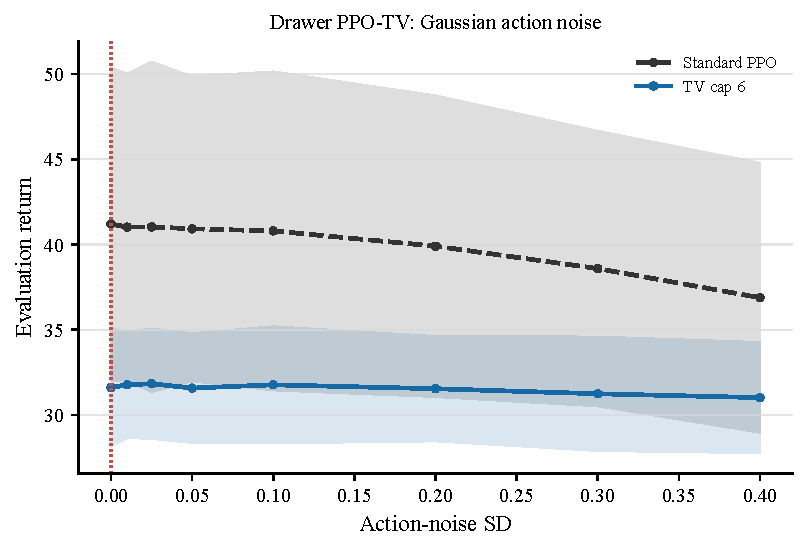
\includegraphics[width=\linewidth]{plots/drawer_ppo_tv30/action_noise.pdf}
\caption{Gaussian action noise}
\end{subfigure}\hfill
\begin{subfigure}{0.48\textwidth}\centering
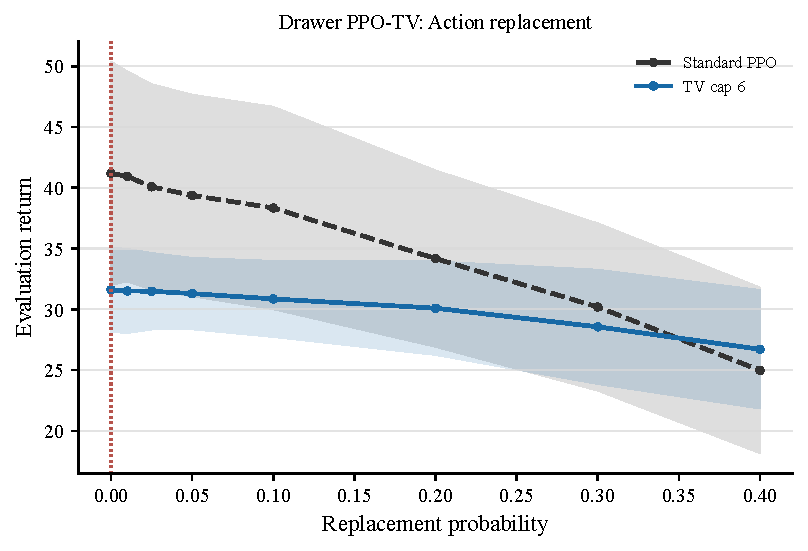
\includegraphics[width=\linewidth]{plots/drawer_ppo_tv30/action_replacement.pdf}
\caption{Action replacement}
\end{subfigure}\par\medskip
\begin{subfigure}{0.48\textwidth}\centering
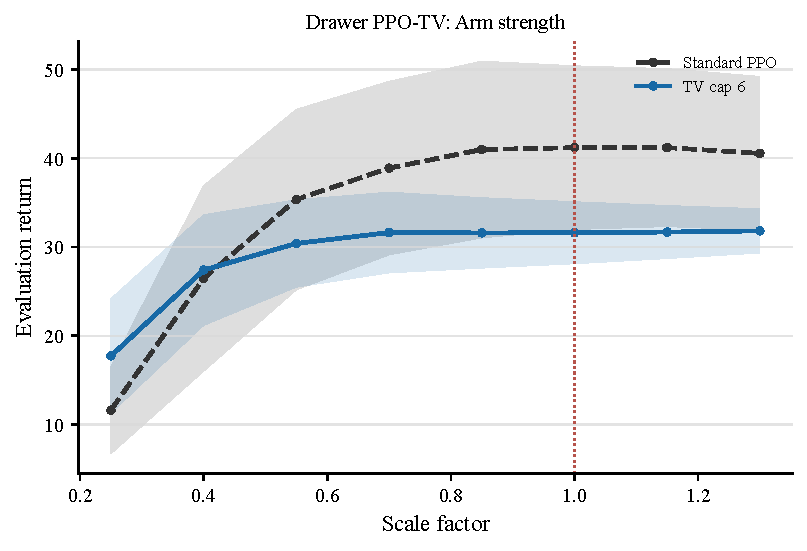
\includegraphics[width=\linewidth]{plots/drawer_ppo_tv30/arm_strength.pdf}
\caption{Arm strength}
\end{subfigure}\hfill
\begin{subfigure}{0.48\textwidth}\centering
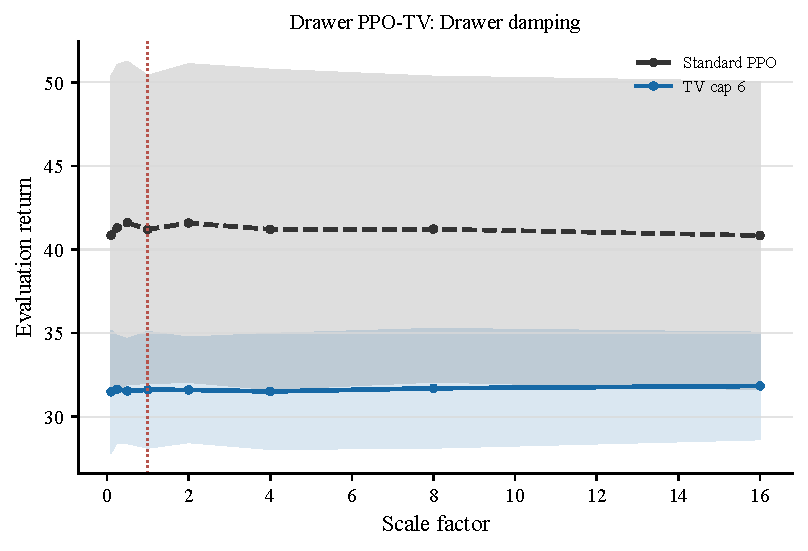
\includegraphics[width=\linewidth]{plots/drawer_ppo_tv30/drawer_damping.pdf}
\caption{Drawer damping}
\end{subfigure}\par\medskip
\caption{Drawer PPO-TV. Mean and sample SD across 30 training seeds; ex-post selection.}
\end{figure}
\begin{figure}[p]\centering
\begin{subfigure}{0.48\textwidth}\centering
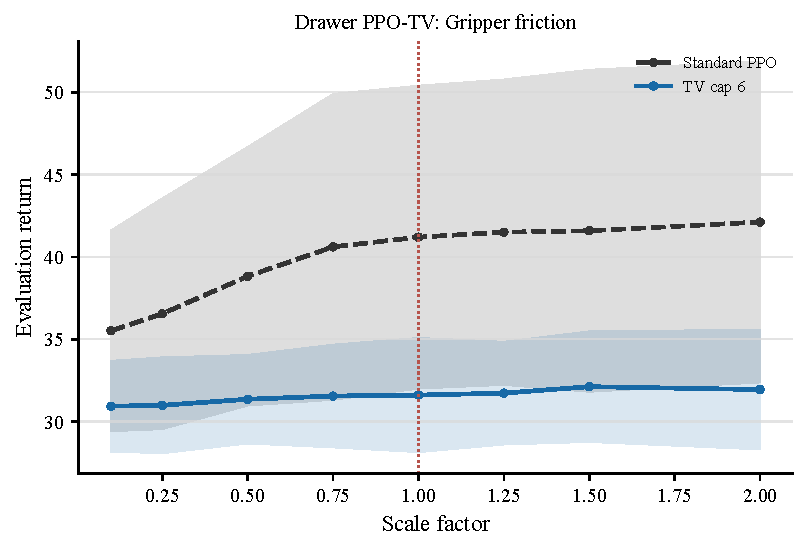
\includegraphics[width=\linewidth]{plots/drawer_ppo_tv30/gripper_friction.pdf}
\caption{Gripper friction}
\end{subfigure}\hfill
\begin{subfigure}{0.48\textwidth}\centering
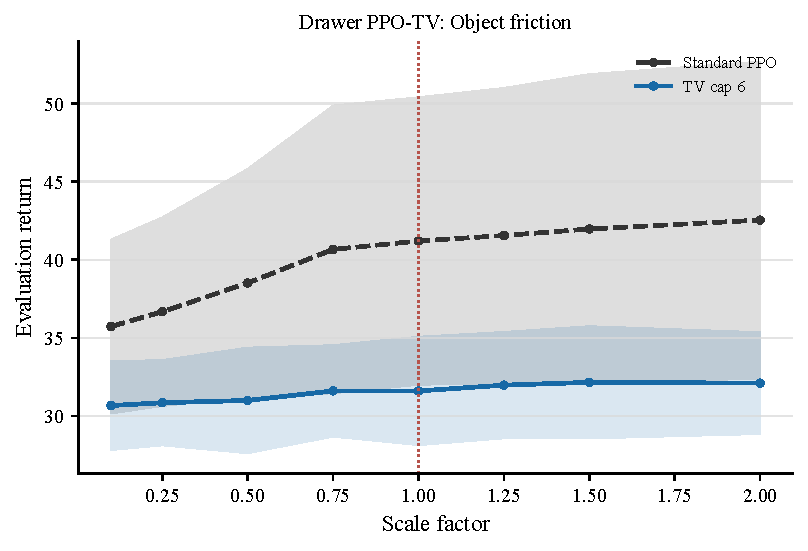
\includegraphics[width=\linewidth]{plots/drawer_ppo_tv30/object_friction.pdf}
\caption{Object friction}
\end{subfigure}\par\medskip
\begin{subfigure}{0.48\textwidth}\centering
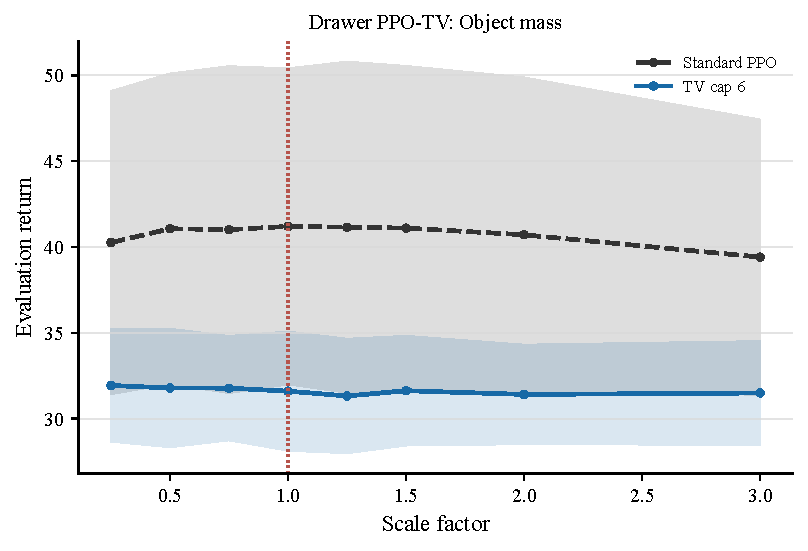
\includegraphics[width=\linewidth]{plots/drawer_ppo_tv30/object_mass.pdf}
\caption{Object mass}
\end{subfigure}\hfill
\caption{Drawer PPO-TV. Mean and sample SD across 30 training seeds; ex-post selection.}
\end{figure}
\subsection{PickCube-v1 SAC-KL}
Thirty training seeds per setting. Bands are one sample SD across policy means, not confidence intervals. Ordinary standard is fixed; the best complete parameter is selected ex post separately per axis. Available full-30 beta settings only; beta 0.1 and 0.3 each retain two failed seeds and are excluded. End-effector-delta 1M-transition recipe; fixed ordinary SAC from the delivered matching cohort. KL bypass retained separately, not certified native parity. No full-grid completion or robust-success claim.
\begin{figure}[p]\centering
\begin{subfigure}{0.48\textwidth}\centering
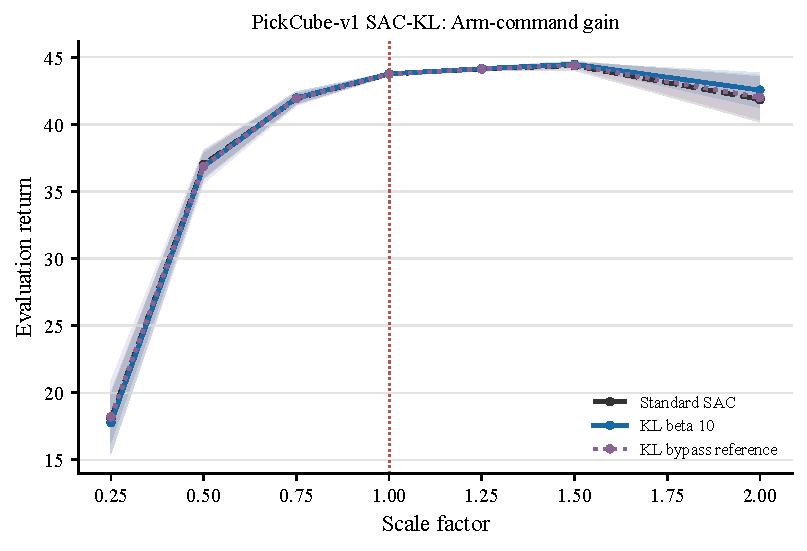
\includegraphics[width=\linewidth]{plots/pickcube_sac_kl30/arm_command_gain.pdf}
\caption{Arm-command gain}
\end{subfigure}\hfill
\begin{subfigure}{0.48\textwidth}\centering
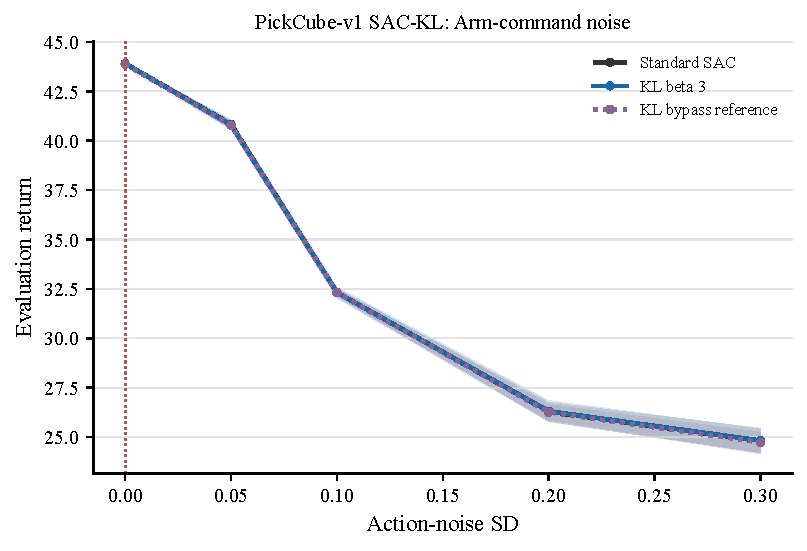
\includegraphics[width=\linewidth]{plots/pickcube_sac_kl30/arm_command_noise.pdf}
\caption{Arm-command noise}
\end{subfigure}\par\medskip
\begin{subfigure}{0.48\textwidth}\centering
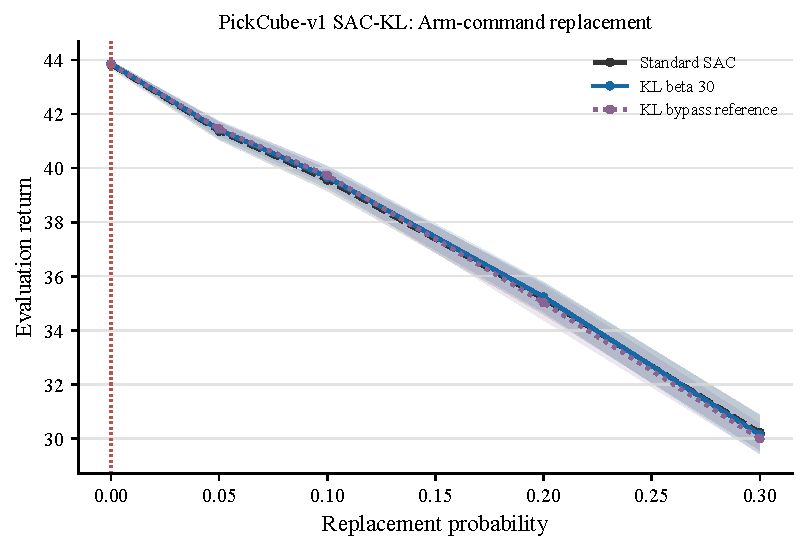
\includegraphics[width=\linewidth]{plots/pickcube_sac_kl30/arm_command_replacement.pdf}
\caption{Arm-command replacement}
\end{subfigure}\hfill
\begin{subfigure}{0.48\textwidth}\centering
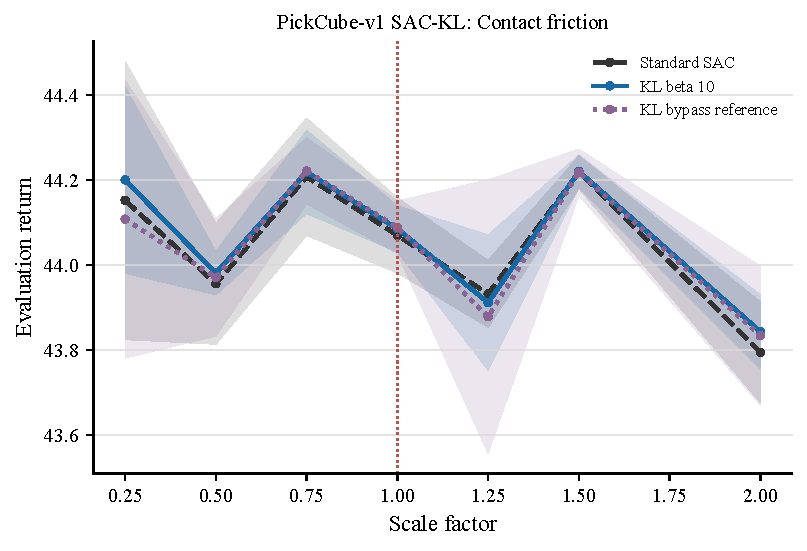
\includegraphics[width=\linewidth]{plots/pickcube_sac_kl30/contact_friction.pdf}
\caption{Contact friction}
\end{subfigure}\par\medskip
\caption{PickCube-v1 SAC-KL. Mean and sample SD across 30 training seeds; ex-post selection.}
\end{figure}
\begin{figure}[p]\centering
\begin{subfigure}{0.48\textwidth}\centering
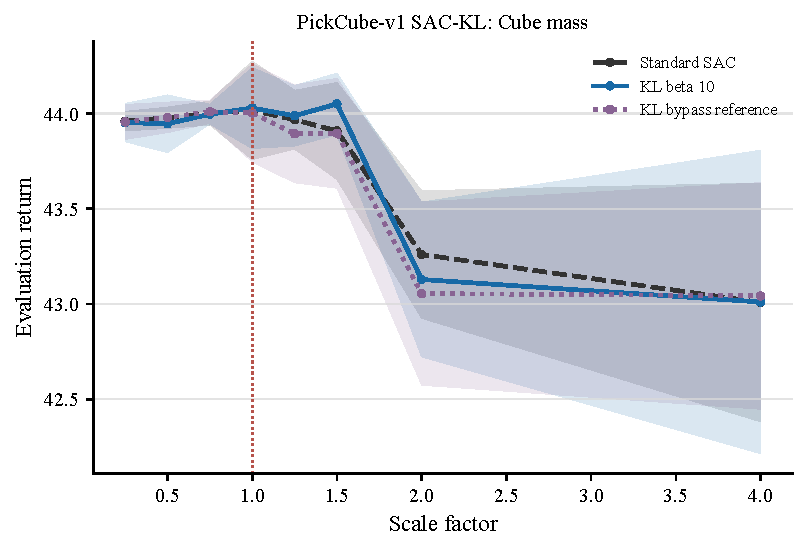
\includegraphics[width=\linewidth]{plots/pickcube_sac_kl30/cube_mass.pdf}
\caption{Cube mass}
\end{subfigure}\hfill
\begin{subfigure}{0.48\textwidth}\centering
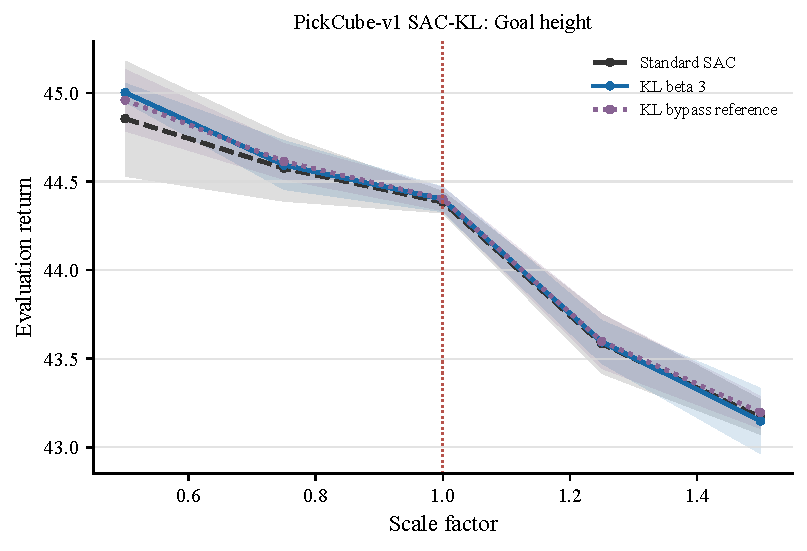
\includegraphics[width=\linewidth]{plots/pickcube_sac_kl30/goal_height.pdf}
\caption{Goal height}
\end{subfigure}\par\medskip
\caption{PickCube-v1 SAC-KL. Mean and sample SD across 30 training seeds; ex-post selection.}
\end{figure}
